%%=============================================================================
%% Methodologie
%%=============================================================================

\chapter{\IfLanguageName{dutch}{Methodologie}{Methodology}}
\label{ch:methodologie}

%% TODO: Hoe ben je te werk gegaan? Verdeel je onderzoek in grote fasen, en
%% licht in elke fase toe welke stappen je gevolgd hebt. Verantwoord waarom je
%% op deze manier te werk gegaan bent. Je moet kunnen aantonen dat je de best
%% mogelijke manier toegepast hebt om een antwoord te vinden op de
%% onderzoeksvraag.

Vooraleer we starten met het uitwerken van de proof of concept, zal er eerst een opsomming worden gemaakt van de nodige requirements. Om het onderzoek succesvol te kunnen uitwerken moet er gezocht worden naar python projecten die voldoen aan bepaalde criteria. 
Deze kunnen we opdelen in functionele en niet-functionele requirements.

\section{Requirements van de proof of concept}

\subsection{Functionele requirements}

Onze proof of concept bestaat uit het uitwerken van een programmeeropdracht via een single board computer die kan gebruikt worden in een les in het secundair onderwijs. Het moet dus voldoen aan de eindtermen van Digitale competentie en mediawijsheid of concreter aan de eigenschappen van computationeel denken, voldoen. Dit betekend dat elk onderdeel makkelijk te vinden is in het project. Zo moet er duidelijk gebruik gemaakt worden van decompositie, abstractie, patroonherkenning en algoritmisch denken binnen het project. Wanneer deze niet aanwezig zijn voldoet het niet aan de eindtermen, opgegeven door het onderwijsdecreet. 

Als tweede functionele requirement moet er gebruik gemaakt worden van de programmeertaal Python om dit project te realiseren. Zoals vermeld in de literatuurstudie is Python een geschikte kandidaat om leerlingen te leren over de basisonderdelen van programmeren. In het project moeten dus de basisinstructies voorkomen. Voorbeelden hiervan zijn bijvoorbeeld het gebruik van lussen en voorwaarden. Hierbij proberen we een zo goed mogelijk beeld te schetsen over hoe applicaties worden gemaakt en hoe een computer precies “denkt”. Ook deze eigenschappen zijn noodzakelijk voor het slagen van dit project.

Een volgende requirement spreekt over de vorm waarin dit project moet worden uitgevoerd . Dit project moet bestaan uit verschillende onderdelen die het proces makkelijker maakt voor een leerkracht om te implementeren in de les. Het moet dus bestaan uit een introductie, een  probleemstelling, het uitvoeren van het project en de conclusie ervan. Er is dus sprake van een rode draad doorheen het gehele proces. Wanneer dit niet op voorhand wordt opgesteld maakt het het moeilijker voor de leerkracht om dit uit te werken. 

Tenslotte bestaat de laatste functionele requirement uit het gebruik van de hardware. Het volledige project moet kunnen worden uitgevoerd op zowel een traditionele computer als een Raspberry Pi. Dit gaat van het opstarten van het project tot het afwerken van het project. Aangezien we een SWOT analyse willen uitvoeren, moet het project op beide hardwares uitgevoerd worden. Deze apparaten moeten ook compleet los van elkaar het project draaien. Het gebruik van bijvoorbeeld een externe pc bij het programmeren van een Pi is verboden. Het installeren van het besturingssysteem van de Pi is geen onderdeel van dit project en zal dus niet opgenomen worden bij de requirements. Wanneer men gebruik moet maken van externe hardware om het project uit te voeren, is het project niet geslaagd.

Nu we een aantal functionele requirements hebben opgesomd, kunnen we een aantal niet-functionele requirements aanhalen. Ook deze zijn belangrijk bij het slagen van het onderzoek.

\subsection{Niet-functionele requirements}

Dit project moet kunnen worden uitgevoerd in lessen van de eerste graad van het secundair onderwijs. Dit betekent dat het project makkelijk te begrijpen moet zijn voor leerlingen van die graad. Het project moet dus kunnen worden uitgelegd met zo min mogelijk vaktermen van de informatica. Het moet dus in andere woorden moeten kunnen uitgelegd worden in het grammaticaal niveau van een twaalf tot veertien jarig kind. Als men te veel vaktermen op voorhand moet uitleggen, maakt het het project niet zo praktisch om uit te voeren in de eerste graad.

Om verder te gaan op de vorige niet-functionele requirement, moet het project kunnen worden voorgelegd in een tijdspanne van 1 tot 2 lesuren. Dit mag dus maximaal twee maal 50 min. duren (1 uur en 40 min.). Aangezien we met een bepaalde structuur werken, moet er dus duidelijk rekening gehouden worden met de benodigde tijd. Als men dit project moet splitsen in verschillende lessen, kan dit moeilijker zijn voor de leerling om de draad opnieuw op te pakken.

Verder moet de leerkracht dit project kunnen uitvoeren zonder of met minimale technische hulp. Om de vlotheid van een les te kunnen bewaren, moeten alle vragen en problemen met gemak kunnen worden opgelost door een leerkracht zonder informatica ervaring. Er moet dus een duidelijke handleiding bestaan bij het uitwerken van het project.

Aangezien een single board computer goedkoop is en open source eigenschappen bevatten, moet het project dit ook reflecteren. Het project moet met andere woorden gratis en open source zijn. Wanneer we te veel geld moeten uitgeven bij het maken van dit project, verliezen we de aantrekkelijke financiële eigenschappen van single board computers. 

Tenslotte moet het project een creatieve ingeving hebben. Omdat we werken met leerlingen uit de eerste graad is het gebruik van een professionele use case niet aantrekkelijk. Het project moet dus uitdagend zijn en leuk om uit te voeren.

\subsection{Samengevat}

Nu we duidelijk een beeld hebben aan wat het project moet voldoen en waaraan het zich moet houden, kunnen we deze nog verder classificeren. Elke requirement heeft een prioriteit. Sommigen zijn cruciaal, terwijl andere de kwaliteit van het project slechts verbeterd. Alle requirements aftikken is niet makkelijk, dus een lijst van must-have’s, should-have’s en nice-to-have’s zou hierbij kunnen helpen.


Figuur \ref{fig:moscow} toont de prioriteit aan van de verschillende requirements.

\begin{figure}
   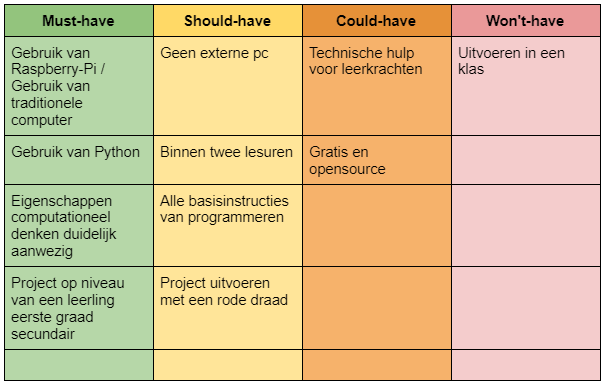
\includegraphics[width=\linewidth]{requirements}
   \caption{MoSCoW voorstelling van de requirements}
   \label{fig:moscow}
\end{figure}

\section{Long list}

Nu we duidelijk weten wat we kunnen verwachten van ons project, kunnen we nu verschillende opties proberen en evalueren of er genoeg requirements afgetikt zijn. Aangezien we al de hardware en software hebben bepaald, kunnen we makkelijk zoeken naar mogelijke projecten. Hiervoor bekijken we volgende opties:

Dankzij de website “upgrad.com” kunnen we al een paar projecten evalueren, zoals het maken van een Tic-tac-toe spel (xox). Dit kan gemaakt worden met behulp van Python en kan zeker gemaakt worden op een Raspberry Pi, maar het programmeerniveau van zo’n applicatie ligt iets te hoog voor beginnende programmeurs. 

Een andere optie is het maken van binair zoekalgoritme. Dit is een klassiek voorbeeld van een basis applicatie. Het tikt dus zeker de box af voor het implementeren van de eigenschappen van computationeel denken en is zeker mogelijk om te maken in Python. Het is echter een minder creatieve opgave en het niveau kan soms al te hoog zijn voor leerlingen van de eerste graad.

Een contactlijst is dan weer een andere optie. Hierin kan iemand contactgegevens opslaan van zijn beste vriend of vriendin. Dit kan zeker gemaakt worden in Python, maar bestaat niet echt uit de basisinstructies van programmeren en kan zelf complexere methodes opvragen. Het lijkt dus geen aantrekkelijke optie.

Dankzij een YouTube video van freeCodeCamp.org kunnen we nog een paar projecten evalueren, zoals het maken van een photo processor. Hierbij kan je een foto aanpassen door het bijvoorbeeld waziger te maken of door de belichting te verhogen. Allemaal via wat lijntjes code. Opnieuw, dit is een project dat men kan maken in Python, maar de onderdelen van computationeel denken zijn vager aanwezig. Er is een kennis van fotobewerking nodig om het probleem makkelijk te onderverdelen in kleinere problemen. Het niveau ligt dus waarschijnlijk iets te hoog.

We kunnen misschien een raadspel maken. Hierin kan de gebruiker dus proberen een getal te raden die de computer heeft gekozen of zelfs een programma maken waarmee het zelf een getal kan raden. De eigenschappen van computationeel denken zitten hier duidelijk in verwerkt. Aangezien het een spel is, heeft het dus zeker een creatieve input. Het lijkt dus een goede optie.

Verder kunnen we misschien een mad libs spel maken. Hierin vraagt de computer om bepaalde woorden zoals bijvoeglijke naamwoorden of werkwoorden die de gebruiker moet ingeven, waarna het een verhaal maakt met de ingegeven woorden. Dit is zeker een creatief project en heeft duidelijk de eigenschappen van computationeel denken in verwerkt, maar het is een wat te makkelijke opgave. Het bevat ook weinig tot bijna geen basisinstructies, zoals een voorwaarde of een lus. Minder aantrekkelijk dus.

Nog een bekend spel dat we zouden kunnen uitwerken in Python, is hangman. Hierin proberen mensen een bepaald woord te raden binnen een bepaald aantal beurten. Op zich lijkt dit een ideaal voorbeeld van een klassieke programmeeroefening. Je kan snel de eigenschappen van computationeel denken herkennen en het bevat de basisinstructies van programmeren. Een goede kandidaat dus.
Tenslotte kunnen we proberen om het klassieke blad steen schaar spel na te maken in Python. Ook hier zijn de eigenschappen van computationeel denken duidelijk aanwezig. Ook heeft het een creatieve input aan het project. Nog een geschikte kandidaat.

Nu we een lijst van potentiële opgaven hebben gemaakt, kunnen we bekijken welke projecten meer geschikt zijn voor zelf uit te voeren. Men kan in vorige oplijsting dus een drietal kandidaten uitvissen: Het getal raad spel, hangman en “blad steen schaar”. Om de meest geschikte kandidaat te bepalen, moeten we volgende projecten verder in detail bespreken.

\section{Short list}

We hebben drie projecten die we kunnen evalueren tegenover elkaar. Er zal een project uitgekozen worden om verder uit te werken in een proof of concept.

\subsection{Hangman}

Hangman is een simpel spel waarin de speler proberen een woord te raden van een medespeler. Zo moeten de speler letters raden die misschien in het woord zitten. Bij elk juist antwoord worden alle plaatsen waarin de letter in het woord verwerkt zit, getoond. Bij elk fout antwoord wordt er een deel van de hangman getekend. Het spel eindigt wanneer alle letters geraden zijn of wanneer de hangman volledig getekend is.

We kunnen alle aspecten van hangman bekijken om te kunnen evalueren of het een geslaagd project kan zijn. Het bevat bijvoorbeeld duidelijk de eigenschappen van computationeel denken. 

Men kan dankzij decompositie het hele spel opsplitsen in verschillende tussen problemen: de gebruiker raad, de computer evalueert de gegeven letter, de computer “tekent” de hangman, de computer controleert als het woord geraden is, de computer toont een letter en het spel eindigt. 

Dankzij abstractie kunnen we deze problemen versimpelen. Bij de eerste stap geeft de gebruiker een letter in. Hierna controleert de applicatie of de letter aanwezig is in het woord. Wanneer de letter aanwezig is toont de applicatie het lege woord met de ingevulde letters. Hierna controleert de applicatie als alle letters geraden zijn.  Als dit zo blijkt te zijn,  stopt het spel en is de gebruiker gewonnen. Anders spelen we verder. Wanneer de letter niet te vinden is, verhogen we de “hangman” teller. Als de teller een boven een vastgelegde waarde zit, zoals bijvoorbeeld zeven, stopt het spel en wint de computer. 

Dankzij patroonherkenning zien we dat deze fases constant herhaald worden tot het spel stopt. Ook zien we duidelijk vier verschillende fases die herhaald worden: de raad-fase, de controle-fase, de uitkomst fase en de “einde spel”-fase. Ook bij de controle-fase gebruik gemaakt van de input van de gebruiker, dus is er sprake van een voorwaarde.

Als we nu al deze fases aan elkaar hangen op een logische manier, hebben we dankzij algoritmisch denken het hangman spel gemaakt.

Juist omdat het een bekend spel is, is er weinig vakjargon die moet aangeleerd worden bij het uitwerken van dit project. Ook maakt het gebruik van meerdere basisinstructies. 

Een probleem bij dit project kan de complexiteit zijn. Er zijn veel stappen die moeten worden doorlopen om het spel te kunnen uitspelen. Dit kan ervoor zorgen dat er sneller problemen kunnen oplopen tijdens het uitwerken in de klas. De handleiding voor de leerkracht zou dus al in lengte groeien. Ook zou het kunnen dat dit project langer dan twee lesuren kan duren, waardoor de vlotheid van het project een deuk neemt. 

Toch is het een goede optie om uit te werken, al dan niet in een langere periode dan twee lesuren. Het is een creatief spel waarmee de leerlingen zeker plezier mee kunnen ervaren.

\subsection{Blad Steen Schaar}

Ook “Blad Steen Schaar” is een leuk spel om te maken op de computer. Als we de eigenschappen van computationeel denken erop laten los gaan, kunnen we bekijken als het genoeg potentieel heeft om verder uitgebouwd te worden.

Via decompositie kunnen we ook dit probleem opdelen in verschillende kleinere problemen: de speler speelt, de computer speelt, de computer evalueert de beide keuzes en een punt wordt gegeven aan de winnaar. Eventueel kan je de “beste uit drie”-regel toepassen het spel laten stoppen binnen drie beurten. Hierbij komt de stap erbij dat de computer controleert als het spel gedaan is.

Via abstractie kunnen we deze deelproblemen verder uitwerken. Bij de eerste stap vraagt de computer om een input van de gebruiker: blad, steen of schaar. Hierna geeft de gebruiker één van deze keuzes in. Hierna kiest de computer een willekeurige zet. In de volgende stap bekijkt de computer dankzij een legende wie gewonnen heeft en geeft de winnaar een punt. Winnaar men binnen drie beurten speelt, kan de computer nog evalueren als het spel afgelopen is. Zo zou het spel stoppen wanneer een van beide partijen een 2-0 heeft of wanneer iemand een hogere score heeft na drie zetten.

Via patroonherkenning zien we in dat er bepaalde fases worden doorlopen: de keuze-fase, de punten-fase en de controle-fase. Deze worden steed opnieuw herhaald. Ook stopt het spel na drie beurten en wordt de input van de gebruiker verwerkt, wat wijst op een voorwaarde. Tenslotte worden deze fases in chronologische volgorde uitgevoerd, ook al kan men beslissen om eerst de computer te laten kiezen en dan pas de gebruiker.
Dankzij algoritmen kunnen deze fases aan elkaar worden gekoppelt voor een volledig resultaat. 

In tegenstelling tot het hangman spel is dit een korter project om uit te werken. Hierdoor is het makkelijker om uit te voeren in de klas en om het binnen de periode van twee lesuren te houden. Dankzij de simpliciteit van “blad steen schaar” is er ook minder uitleg nodig voor leerlingen en leerkrachten.

Deze simpliciteit heeft echter zijn nadelen. “Blad steen schaar” is nogal simpel en misschien niet zo interessant voor leerlingen om zich daar twee lesuren mee bezig te houden. Maar zelfs met de negatieve aspecten lijkt blad steen schaar een goede keuze om te gebruiken tijdens de lessen computationeel denken.

\section{Proof of concept: Raadspel}

De proof of concept voor dit onderzoek bestaat uit het opstellen van een lesvoorbereiding voor het raadspel met gebruik van Python en een Raspberry Pi. Hierna zal de uitvoering van de lesvoorbereiding gemaakt worden op zowel een traditionele computer als een Raspberry Pi. Hieruit kunnen we een SWOT-analyse opstellen en evalueren of de Raspberry Pi een meerwaarde geeft in de lessen programmeren in de eerste graad van het secundair onderwijs.

\subsection{Lesvoorbereiding}
Als deel van de proof of concept, wordt er een lesvoorbereiding gemaakt voor het maken van een Raadspel. Dit zal volledig gemaakt worden in Python en zal in de SWOT-analyse uitgevoerd worden op zowel een Raspberry Pi als een klassieke computer. Hieruit zullen we kunnen bekijken wat de gebruikerservaring van een Pi is.

Om een project om te vormen naar een lesactiviteit, is een lesvoorbereiding van cruciaal belang. Alleen zo geef je een project wat structuur en maak je het makkelijker voor de leerkracht om te evalueren als je opdracht alle einddoelen aftikt.

[WORK IN PROGRESS]

\subsection{SWOT-analyse Raspberry Pi}

Zoals eerder vermeld heeft, bestaat de proof of concept uit een vergelijking met traditionele computers zoals een desktop of laptop. Hiervoor zullen dezelfde stappen uitgevoerd worden op zowel de Pi als de klassieke computer. Beide scenario’s worden los van elkaar uitgevoerd, maar moeten identiek en repliceerbaar zijn.


We belichten eerst de sterke eigenschappen van het programmeren met een Pi. 
Het startscherm van de Raspberry Pi is enorm herkenbaar in vergelijking met andere besturingssystemen. Er was geen nood aan het opzoeken van een handleiding om te kunnen starten. Dankzij de duidelijke gebruikersinterface kan je makkelijk de ingebouwde browser vinden, een tekstbestand opstellen, files aanmaken, uw mappen organiseren en veel meer. Het aanpassen van de schermresolutie was ook intuïtief. Alle interactie schermen zijn minimalistisch en to-the-point. Wanneer men toch hulp nodig heeft, kan je makkelijk een handleiding aanroepen via het startmenu, te herkennen aan het Raspberry logo in de taakbalk. Dit maakt het besturingssysteem aanzienlijk gebruiksvriendelijker dan klassieke UI’s, zoals Microsoft Windows, die soms met hun vele features de gebruikers kan afschrikken.

Voor dagdagelijkse praktijken zoals een word document opstellen, kan je snel de “Office”-knop indrukken in het startmenu om de Pi variant van Microsoft Office te gebruiken: LibreOffice. Deze applicaties zijn gratis en komen geïnstalleerd bij het besturingssysteem. Dit komt steeds minder vaak voor in de wereld van de klassieke computers. Bij Windows moet men zelf betalen voor deze features. Dit maakt de Raspberry Pi een interessante concurrent op vlak van office-tools.

De Raspberry Pi OS maakt het makkelijk om snel een project te starten via de startmenu. Door door te klikken op de programmeren optie kan je makkelijk Thonny vinden en opstarten. Klassieke besturingssystemen hebben vaak geen voorgeïnstalleerde IDE. De instapklare eigenschap van de Pi is dus zeker een pluspunt. 

Zoals eerder vermeld, wordt er gebruik gemaakt van Thonny: een gebruiksvriendelijke en simpele IDE die standaard geïnstalleerd is op de Raspberry Pi OS. Deze IDE maakt gebruik van een duidelijk en minimalistische gebruikersinterface om zo snel mogelijk van slag te gaan. Je krijgt meteen twee schermen te zien: het script en de shell. Via het script kan je makkelijk je project beginnen programmeren en via de shell kan je het script runnen. Er zitten ook handige features in zoals een debug mode en een code correctie hulp die u code controleert en feedback geeft over wat er beter kan. 

De gebruikerservaring bij het programmeren zelf is praktisch en gestroomlijnd. Dankzij de snelknoppen naar de IDE en de simpele gebruikersinterface kan je snel een project opstarten en uitvoeren.


De Pi toont zijn lelijke kantjes wanneer je het wilt gebruiken voor meer dan simpele programmeer sessies. Dankzij zijn gelimiteerde hardware en features kan de gebruikservaring snel dalen wanneer je een Pi gebruikt voor meer alledaagse activiteiten zoals youtube video’s bekijken. Door de gelimiteerde hardware kan de Pi moeilijk image en video processing aan, waardoor youtube video’s vaak haperen en streaming praktisch onmogelijk lijkt.

Zoals vermeld heeft de Pi al verschillende, voorgeïnstalleerde programma’s voor dagdagelijkse activiteiten zoals LibreOffice, maar ook deze hebben problemen. De gebruikersinterface lijkt enorm gedateerd en onaantrekkelijk. Door het gebruiksvriendelijk te maken worden vaak vele handige features geschrapt. Het mist bijvoorbeeld veel layout opties die standaard zijn bij Word, zoals het vrij aanpassen en toevoegen van stijlen. 
Dit probleem is niet enkel te zien bij LibreOffice. Heel wat onderdelen van het besturingssysteem voelen gedateerd en gelimiteerd aan. 

Dankzij de gelimiteerde hardware is de Pi ook gevoelig aan lag: het proces waarbij programma's trager aanvoelen of vaak blokkeren. Tijdens het gebruik van de browser kan men vaak langer wachten op zoekresultaten dan bij een klassieke browser. Ook dit heeft een negatief effect op de gebruikerservaring van de Pi.

De grootste slag in het gezicht bij de Pi is iets wat je niet direct zou aan denken met een klassieke pc, maar toch o zo belangrijk is: de stroomtoevoer. Aangezien de Pi zijn stroomtoevoer krijgt van een USB-C of Micro-USB kabel, is het gevoelig aan wisselingen in voltage. Bij het opladen van een gsm is dit minder merkbaar, maar bij het volledig draaien van een computer is dit duidelijk merkbaar. Wanneer de Pi detecteert dat er te weinig stroomtoevoer binnen vloeit in het apparaat, geeft het een melding die om de vijf minuten terugkeert. Hierbij vraagt het om uw Raspberry Pi te verbinden met een sterkere stroombron. Dit kan echter aan veel onderdelen liggen, van de adapter waarmee je het in het stopcontact steekt tot het stopcontact in kwestie. Het is dus onvoorspelbaar als uw Pi genoeg stroom zal krijgen om te blijven doorwerken.

Maar zoals je waarschijnlijk al denkt, is de melding het minste van je zorgen. Wanneer de Pi te weinig activiteiten tegelijk moet draaien op een lage energiebron, kan het spontaan uitvallen en opnieuw opstarten. Dit heeft een drastisch effect op je workflow en de gebruikerservaring. Wanneer de Pi opnieuw opstart, kan het niet garanderen dat al uw werk van vooraf opgeslagen blijft. Hierdoor kan de gebruiker uren van werk kwijtraken. 
Maar dit is nog niet het ergste aspect van een stroomuitval. Zoals vermeld in de literatuurstudie, heeft de Pi geen functie waarbij het lopende processen eerst afsluit voordat het stroom verliest. Hierdoor kan niet enkel uw files beschadigt raken, maar zelfs uw hele besturingssysteem, waardoor je al uw werk compleet kan kwijtraken. Dit is een gigantische dreun in het gezicht van de Raspberry Pi.  

Los van deze tekortkoming heeft de Pi toch nog kansen om verder uit te groeien naar een goede substitutie voor een klassieke computer in de klassfeer. De Raspberry Pi foundation en zijn actieve community zijn nog altijd bezig met het verbeteren van de Pi ervaring. Er komen nog steeds nieuwe modellen op de markt, met de Pi 400 speciaal ontworpen om de normale desktop of laptop te vervangen. Met de jaren kunnen we betere prestatie verwachten en zou het weleens een rol kunnen spelen in het onderwijs.
Zoals vermeld zijn er actieve communities die ofwel proberen het bestaande besturingssysteem te optimaliseren oftewel totaal nieuwe besturingssystemen introduceren zoals Linux. 

De Pi vecht momenteel wat tegen de bierkaai als het probeert om traditionele computers te vervangen. Eenmaal het verbeterd in prestaties of grafische capaciteiten, zijn klassieke pc’s al uitgerust met nog nooit geziene snelheden en prestaties. Ook genieten single board computers nog niet van de bekendheid die moderne smart apparaten wel hebben. Het blijft een wat nich concept voor velen. Zoals eerder vermeld bij het kiezen van een single board computer zijn leerkrachten nog niet overtuigd om het te implementeren in de klas.




